\documentclass[twoside,a4paper,10pt]{report}
%%\usepackage[french]{babel} %% Use your own babel language
\usepackage[top=3cm,bottom=3cm,left=2.5cm,right=2.5cm]{geometry}
\usepackage{ucs}
\usepackage[utf8x]{inputenc}
\usepackage{pslatex}
\usepackage{hyperref}
\usepackage{graphicx}
\usepackage{tabularx}
\usepackage{supertabular}
\usepackage{pdflscape} %% Used for very big table
\usepackage{pdfpages} %% To add a cover to the doc
\usepackage{moreverb}
\usepackage{xcolor}
\usepackage{listings}
\usepackage{lastpage}
\usepackage{fancyhdr}
\usepackage{ulem}
\usepackage{textcomp}
\usepackage{wasysym}
\usepackage{sectsty}
\usepackage{wrapfig} %%Usefull for image 
%\usepackage{fguill} %%Use this package for guillemot[left|right] useless with babel set to french
\usepackage{eso-pic} %% Background
\pagestyle{fancy}%
\renewcommand{\headrulewidth}{0.1pt}
\renewcommand{\footrulewidth}{0pt}
\renewcommand{\chaptermark}[1]{%
	\markboth{\sffamily \chaptername\ \thechapter.\ #1}{}}

\renewcommand{\sectionmark}[1]{%
	\markright{{\sffamily #1}}{}}

\fancypagestyle{plain}{%
\fancyhf{}
\fancyfoot[R]{\thepage/\pageref{LastPage}}
\renewcommand{\headrulewidth}{0pt}
\renewcommand{\footrulewidth}{0pt}}
\fancyhf{}
\fancyhead[L]{\rightmark}
\fancyhead[R]{\leftmark}
\fancyfoot[R]{\thepage/\pageref{LastPage}}
\renewcommand{\headrulewidth}{0.1pt}
\renewcommand{\footrulewidth}{0pt}

\definecolor{Light}{gray}{.80}
\definecolor{Dark}{gray}{.20}

\newcommand{\key}[1]{\fcolorbox{Dark}{Light}{\textbf{#1}}}

\newcommand{\settexitref}[2]{(\ref{#1}p\pageref{#1})}
\newcommand{\dokutitlelevelone}[1]{\chapter{#1}}
\newcommand{\dokutitleleveltwo}[1]{\section{#1}}
\newcommand{\dokutitleleveltree}[1]{\subsection{#1}}
\newcommand{\dokutitlelevelfour}[1]{\subsubsection{#1}}
\newcommand{\dokutitlelevelfive}[1]{\paragraph{#1}}
\newcommand{\dokufootnote}[1]{\footnote{#1}}
\newcommand{\dokufootmark}[1]{\footnotemark[#1]}
\newcommand{\dokubold}[1]{\textbf{#1}}
\newcommand{\dokuitalic}[1]{\textsl{#1}}
\newcommand{\dokumonospace}[1]{\texttt{#1}}
\newcommand{\dokuunderline}[1]{\underline{#1}}
\newcommand{\dokuoverline}[1]{\sout{#1}}
\newcommand{\dokusupscript}[1]{\textsuperscript{#1}}
\newcommand{\dokusubscript}[1]{$_{#1}$}
\newcommand{\dokuhline}{\line(1,0){400}}
\newcommand{\dokulabel}[1]{\label{#1}}
\newcommand{\dokuitem}{\item}
\newcommand{\dokuquoting}{\textbar}
\newcommand{\dokutabularwidth}{\textwidth}
\newcommand{\dokusupertabularheadbreak}{\small\sl continued from previous page}
\newcommand{\dokusupertabulartailbreak}{\small\sl continued on next page}
\newcommand{\dokuheadingstyle}[1]{\textbf{#1}}
\definecolor{dokuheadingcolor}{rgb}{0,0,0.60}
\newcommand{\dokubackground}[1]{%
\AddToShipoutPicture{%
  \AtTextCenter{%
    \makebox(0,0)[c]{\resizebox{\textwidth}{!}{%
      \rotatebox{25}{\textsf{\textbf{\textcolor[gray]{0.90}{#1}}}}}}%
  }%
 }%
}

\graphicspath{{media/}}

\hypersetup{
pdftitle = {The Modular OpenRobots Simulation Engine - Developers guide},
pdfauthor = {LAAS-CNRS - ONERA},
pdfkeywords = {simulation, blender, robotics},
pdfcreator = {DokuTeXit},
pdfproducer = {dokuwiki + TeXit + pdflatex}
}
\title{The Modular OpenRobots Simulation Engine - Developers guide}
\author{LAAS-CNRS - ONERA}
\date{@DATE@}
\dokubackground{@BGTEXT@}
\begin{document}
\sffamily
\allsectionsfont{\sffamily}

\IfFileExists{cover.pdf}{
\includepdf[pages=-, fitpaper]{cover.pdf}
\thispagestyle{empty}
\cleardoublepage
}

\thispagestyle{empty}
\maketitle
\thispagestyle{empty}
\cleardoublepage
\tableofcontents
\newpage
\thispagestyle{plain}
\cleardoublepage
\newpage
%Rendering morse:dev:summary
\dokuitalic{Uncomment these line to display the "generate PDF\dokufootnote{Portable Document Format}" button that allow to fetch
}the TEX source


\begin{figure*}[h]
\centering

\includegraphics[width=50pt]{openrobots-simulator.png}
\caption{Logo MORSE}
\end{figure*}




\dokutitlelevelone{Developers documentation}
\label{cdb0de77c6812018f32abbd4e86045e9}%% developers_documentation
\label{a80da1282f2c775bbc5f2c92c836968b}%%Start: summary => /home/slemaign/openrobots/data/pages/summary.txt

\dokutitleleveltwo{Get involved!}
\label{9250253a562d7334a71ae2812a91d3bd}%% get_involved

You can write to the list of developers of the project, writing to this address: mailto:morse-dev@laas.fr.

MORSE developement can be tracked online with CGIT: \href{http://trac.laas.fr/git/morse}{ MORSE on CGIT}

You can as well fetch the latest version of the code with GIT:



\lstset{language=TeX}
\begin{lstlisting}
$ git clone http://trac.laas.fr/git/robots/morse.git

\end{lstlisting}
Easy installation instructions will be added after the official release of MORSE 0.1.


\dokutitleleveltwo{Overview}
\label{bce059749d61c1c247c303d0118d0d53}%% overview
An overview of code organization in MORSE

\hyperref[1f96d32f5afc29e1f5142ae3365d880b]{ Overview for MORSE organization}


\dokutitleleveltwo{Workflow}
\label{2e2e2d35a15a6146a9bbbc246a9ea4cd}%% workflow
Principle of interaction with Blender and the game engine

\hyperref[8e26c06a643302a6445b3bace01e145d]{ Overview for MORSE workflow for developers}


\dokutitleleveltwo{Adding a new component}
\label{d6803cd830a74126c504056aa5dc3942}%% adding_a_new_component
Create a sensor. Explain the logic

\hyperref[a75d8217092912ac621cdbf4c37d0162]{ Tutorial: Adding a new component}


\dokutitleleveltwo{With an example of a modifier}
\label{c40195b9cfea7b29114ccb28ad6dc60e}%% with_an_example_of_a_modifier

EZ if in python, a bit more complex if we call an external library (cf impact on the dependencies) 

\hyperref[ddaae98df566ec14d90bd06e83e3787f]{ Tutorial: Creating a modifier}

%Rendering morse:dev:dev_overview
\dokutitlelevelone{A MORSE organization overview}
\label{3317db1fdc670ed991ca495fec5177d0}%% a_morse_organization_overview
\label{1f96d32f5afc29e1f5142ae3365d880b}%%Start: dev_overview => /home/slemaign/openrobots/data/pages/dev_overview.txt

\dokutitlelevelfour{Files hierarchy}

The source code of Morse is organised in the following way :


\begin{itemize}
\dokuitem  bin : it contains the main entry point of the morse simulation
\dokuitem  config : it contains stuff for CMake 
\dokuitem  data : it contains the blender model of sensors / actuators
\dokuitem  doc : the documentation (in DokuWiki format)
\dokuitem  examples : it contains examples about :
\begin{itemize}
\dokuitem  how to control the simulator (in clients)
\dokuitem  more or less elaborate scenarii (in scenarii)
\end{itemize}

\dokuitem  src : it contains all the python scripts used by the simulator : it is the core of the simulator
\dokuitem  morse/actuators : it contains implementation for various robot controllers
\dokuitem  morse/blender : it contains some scripts needed at the initialization of the game engine
\dokuitem  morse/helpers : it contains various helpers (math transformation) and base classes
\dokuitem  morse/middleware : it contains the code for linking with different middlewares 
\begin{itemize}
\dokuitem  yarp
\dokuitem  pocolibs 
\dokuitem  socket
\dokuitem  text (for logging)
\end{itemize}

\dokuitem  modifiers : it contains implementation for various modifier to basic components
\dokuitem  robots : it contains instantiation of different robot classes
\dokuitem  sensors : it contains implementation for various robot sensors
\end{itemize}

\dokutitlelevelfour{Code organization}

The following diagram shows the class hierarchy currently used in MORSE.

\begin{figure*}[h]
\centering
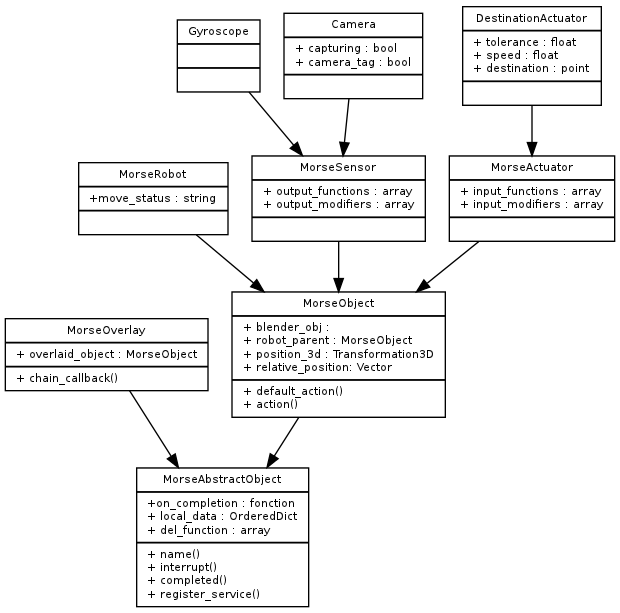
\includegraphics{morse_uml.png}
\end{figure*}


The main entry point for Blender for each component is the method \dokumonospace{action}.
Yet, it is not supposed to be overridden by leaf-classes. To modify the
behaviour of a component, you need to modify the method \dokumonospace{default{\textunderscore}action}. The
action of \dokumonospace{action} depends if it is a sensor or an actuator (robot doesn't do
anything by themself). 


\dokutitlelevelfive{Behaviour of a sensor}

When Blender calls the method \dokumonospace{action} for a sensor, the following things
happen :


\begin{enumerate}\dokuitem  update of the position of the sensor
\dokuitem  call \dokumonospace{default{\textunderscore}action}
\dokuitem  apply in order each function of \dokumonospace{output{\textunderscore}modifiers} (modify the content of the sensor)
\dokuitem  apply in order each function of \dokumonospace{output{\textunderscore}functions} (output the content of the sensor to different clients)
\end{enumerate}

\dokutitlelevelfive{Behaviour of an actuator}

When Blender calls the method \dokumonospace{action} for an actuator, the following things
happen :


\begin{enumerate}\dokuitem  apply in order each function of \dokumonospace{input{\textunderscore}functions} (receive input from different clients)
\dokuitem  apply in order each function of \dokumonospace{input{\textunderscore}modifiers} (if needed)
\dokuitem  call \dokumonospace{default{\textunderscore}action}
\end{enumerate}

Another interesting point is the \dokumonospace{local{\textunderscore}data} dictionary : it contains a
representation of the external state of the sensor (or the actuator) (for
example, it will contains the position for a GPS)

%Rendering morse:dev:dev_workflow
\dokutitlelevelone{The MORSE workflow for developers}
\label{e94f34704efddc910497ce79fd4576f3}%% the_morse_workflow_for_developers
\label{8e26c06a643302a6445b3bace01e145d}%%Start: dev_workflow => /home/slemaign/openrobots/data/pages/dev_workflow.txt

The internal functioning of MORSE is based on Blender's Game Engine events.
These are defined in the Logic buttons window, using the graphical interface called "Logic Bricks". These are a set of predefined \dokubold{Sensor}, \dokubold{Controller} and \dokubold{Actuator} events which can be linked together.
\dokubold{Actuators} in particular are important because they are the places where Python scripts are called.

For Blender to find the Python scripts refered to in the Actuators, the Python files must be directly in a directory listed in \dokumonospace{PYTHONPATH}. The standard location for these files in MORSE is the directory: \dokumonospace{ORS{\textunderscore}ROOT/src/morse/blender}, which should be included in \dokumonospace{PYTHONPATH} as described in the \hyperref[ea09bb364ef1bffd889e76b7a59035fc]{ MORSE installation documentation}.

Each object in Blender can have its own set of Logic Bricks. In every MORSE simulatino scene, there must be one \dokumonospace{Scene{\textunderscore}Script{\textunderscore}Holder} object, which holds the predefined Logic Bricks necessary to initialize and control the simulation.
When a simulation is started (when launching the Game Engine) it will call the initialization scripts of MORSE, contained in the file \dokumonospace{{\textdollar}ORS{\textunderscore}ROOT/src/morse/blender/main.py}.

The script \dokumonospace{main.py} is charged of multiple tasks:


\begin{itemize}
\dokuitem  Upon lanching the simulation, it will initialize all components:
\begin{itemize}
\dokuitem  Create a dictionary of robots
\end{itemize}

\dokuitem  Create a dictionary of components, and the robot their are associated with
\dokuitem  Create the dictionary of modifiers
\dokuitem  Create the dictionary of middlewares
\dokuitem  Link the modifiers and middlewares to components, as specified in the file \dokumonospace{component{\textunderscore}config.py}
\dokuitem  When the simulation ends, it will destroy the objects created, and call the methods to cleanup ports, files, connections, etc.
\end{itemize}

The initialization of all components, including middlewares and modifiers, is done by instantiating an object of the Python class specific to every component. This is done dynamically, using the \dokubold{Class} and \dokubold{Path} properties that should be present in the Blender file of every component.


\dokutitleleveltwo{Events during a simulation}
\label{fefdb00464c51c19fc057196c0844e71}%% events_during_a_simulation

Blender's Game Engine is set to work at a predefined \dokumonospace{Tickrate}, which is the number of times the Logic Brick events are executed per second. In the default settings, it is equal to 60, so that during one real second there will be 60 "ticks".

While the simulation is running, the Logic Bricks of each component will make regular calls to their \dokumonospace{default{\textunderscore}action} method. At this point the component will perform its task and update its internal data.

%Rendering morse:dev:adding_component
\dokutitlelevelone{Adding a new component}
\label{d6803cd830a74126c504056aa5dc3942}%% adding_a_new_component
\label{a75d8217092912ac621cdbf4c37d0162}%%Start: adding_component => /home/slemaign/openrobots/data/pages/adding_component.txt

Each component is basically represented by two files, which must be created when adding a new sensor or actuator:


\begin{itemize}
\dokuitem  A Blender file: has the representation of the sensor on blender, and associate the script with the blender object
\dokuitem  A Python script: contains the logic of the sensor
\end{itemize}

\dokutitleleveltree{The python part}
\label{2f9b01df4a2ece7b3e7028707b901d5f}%% the_python_part

You need to implement a sub-class of \dokumonospace{morse.helpers.sensor.MorseSensorClass} (respectively of \dokumonospace{morse.helpers.actuator.MorseActuatorClass})

Important things to do :


\begin{itemize}
\dokuitem  in the constructor of the object (\dokumonospace{{\textunderscore}{\textunderscore}init{\textunderscore}{\textunderscore}}) :
\dokuitem  initialize each variable you want to expose to the world into \dokumonospace{local{\textunderscore}data}
\dokuitem  initialize correctly \dokumonospace{data{\textunderscore}keys} with the set of variable exposed in \dokumonospace{local{\textunderscore}data} : the order is important here, because this order will be used for the automatic serialization
\dokuitem  initialize correctly \dokumonospace{modified{\textunderscore}data}, with a copy of \dokumonospace{local{\textunderscore}data} (the easiest way is to copy-paste the following code)
\end{itemize}

\lstset{language=python}
\begin{lstlisting}
for variable in self.data_keys:
	self.modified_data.append(self.local_data[variable])

\end{lstlisting}

\begin{itemize}
\dokuitem  override \dokumonospace{default{\textunderscore}action} : it must contains the logic of our component. Avoid to do some big computation here : the function is called often, and it will slow down the whole processing of the Game Engine
\end{itemize}

\dokutitleleveltree{The blender part}
\label{c3a87dbfd0ec95fd40fcfbb5cbd7f50f}%% the_blender_part

\begin{enumerate}\dokuitem  First, create a nice modelling of your object, and save it in \dokumonospace{{\textdollar}MORSE{\textunderscore}ROOT/data/morse/components/sensors/}
\dokuitem  Press \key{N} to display the properties of the object. Change its name.
\dokuitem  Press \key{F4} to enter in the logic mode
\begin{enumerate}\dokuitem  Add the two following properties:
\begin{itemize}
\dokuitem  \dokubold{Class} of type string, which contains the name of the associated python class $<$Sensor$>$Class
\dokuitem  \dokubold{Path} of type string, which contains the path to the associated python script \dokumonospace{morse/sensors/$<$Sensor$>$}	 
\end{itemize}

\dokuitem  You can add more properties if needed for your components. Additional properties can be used to configure the behaviour of the component, and can be integrated into a GUI\dokufootnote{Graphical User Interface} in future versions of MORSE.
\end{enumerate}

\end{enumerate}

The names specified in the \dokubold{Path} and \dokubold{Class} properties must match exactly the location of the Python file and the name of the defined class, respectively.The information in these variables will be used to dinamically load the module and class during initialisation of the simulation.


\dokutitleleveltwo{Getting data or exporting data}
\label{25ef0239968ec09d3b173110a151ecdc}%% getting_data_or_exporting_data

A component is not really useful if it doesn't get any input (for an actuator)
or if you can't use the output of a sensor. You can use different middleware to
import / export data. 

In the simplest case, you can use automatic serialization, which will try to convert the data in \dokumonospace{modified{\textunderscore}data} array into the appropriate format to send throug the middleware. This works only for the basic data types of integer, float or string.
If you want more specific behaviour for other data types, you need to add a method to the middleware provider of your choice
(for example, if you want to export a new sensor through YARP, you need to add
a method to MorseYarpClass, in \dokumonospace{{\textdollar}MORSE{\textunderscore}ROOT/src/morse/middleware/yarp{\textunderscore}mw.py}). The method must have the following prototype :


\lstset{language=python}
\begin{lstlisting}
def your_method(self, component_instance)

\end{lstlisting}
In this method, you can access / store component information through its array
\dokumonospace{modified{\textunderscore}data}. In case of a sensor, it is not expected that you change the
content of the sensor, but only read information in this array.

After that, you need to register your new function into the middleware
abstraction.  For that, you need to modify the method \dokumonospace{register{\textunderscore}component}.
It is basically a switch case with the different possible functions. This
method is called when parsing the configuration file for the scene, so
it is the right place to initialize stuff (opening Yarp ports, sockets, files
\ldots{})


\dokutitleleveltree{Middleware specific information}
\label{908d8d85012025682a1a1a2659804af7}%% middleware_specific_information

\dokutitlelevelfive{YARP}

In MorseYarpClass, the different port{\textunderscore}name are stored in a dictionary
\dokumonospace{{\textunderscore}component{\textunderscore}ports}, indexed by the name of the component
(\dokumonospace{component.blender{\textunderscore}obj.name}). You can retrieve the associated port with the method \dokumonospace{getPort(port{\textunderscore}name)}

Example:



\lstset{language=python}
\begin{lstlisting}
port_name = self._component_ports[component_instance.blender_obj.name]

try:
	yarp_port = self.getPort(port_name)
except KeyError as detail:
	print ("ERROR: Specified port does not exist: ", detail)
	return

\end{lstlisting}

\dokutitlelevelfive{Pocolibs}

In MorsePocolibsClass, the different poster{\textunderscore}id are stored in a dictionary
\dokumonospace{{\textunderscore}poster{\textunderscore}dict}, indexed by the name of the component
(\dokumonospace{component.blender{\textunderscore}obj.name})


\dokutitlelevelfive{Text}

In TextOutClass, the different files are stored in a dictionary
\dokumonospace{{\textunderscore}file{\textunderscore}list}, indexed by the name of the component
(\dokumonospace{component.blender{\textunderscore}obj.name})

%Rendering morse:dev:adding_modifier
\dokutitlelevelone{Creating a modifier}
\label{7ab0c580b65197ee03abbb17c8fa4241}%% creating_a_modifier
\label{ddaae98df566ec14d90bd06e83e3787f}%%Start: adding_modifier => /home/slemaign/openrobots/data/pages/adding_modifier.txt

Creating a modifier is more or less the same than creating a sensor. There are
still two parts, the blender part and the python logic. For the blender part,
it is the same thing than for a sensor / actuator.


\dokutitlelevelfour{Python part}

There is no strict class hierarchy for modifiers, we rely on python duck
typing. We only expect than a modifier exposes a method \dokumonospace{register{\textunderscore}component},
similarly to middleware, with the following prototype :


\lstset{language=python}
\begin{lstlisting}
def register_component(self, component_name, component_instance, mod_data)

\end{lstlisting}
The method is responsible to add the right modifier specified in \dokumonospace{mod{\textunderscore}data}
in the list of modifier of \dokumonospace{component{\textunderscore}instance} ( input{\textunderscore}modifiers or
output{\textunderscore}modifiers ). 

Modifier functions must have the prototype


\lstset{language=python}
\begin{lstlisting}
modifier(self, component_instance)

\end{lstlisting}
In your modifier function, you must only access to the array \dokumonospace{modified{\textunderscore}data}
of the component.

\href{http://trac.laas.fr/git/morse/tree/src/morse/modifiers/gps_noise.py}{GPS{{\textbackslash}textunderscore}noise.py} shows a simple example for a modifier.

\end{document}

